\begin{figure}[h] 
\centering 
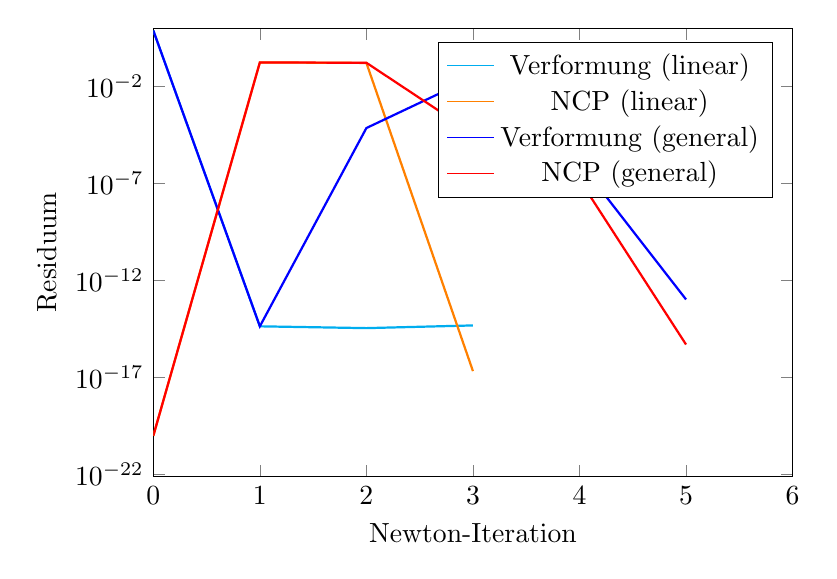
\begin{tikzpicture}[every plot/.append style={thick}] 
\begin{axis}[ 
label style={font=\normalsize}, 
xlabel={Newton-Iteration}, 
ylabel={Residuum}, 
xmin=0, xmax=6, 
ymode=log, 
ymin=0, ymax=10, 
width=0.8\textwidth, 
height=0.6\textwidth, 
legend pos=north east, 
legend style={cells={align=left}}, 
grid style=dashed, 
] 
\addplot[ 
color=cyan, 
] 
coordinates { 
(0, 7.64e+00)(1, 4.37e-15)(2, 3.53e-15)(3, 4.86e-15)}; 
\addlegendentry{Verformung (linear)} 
\addplot[ 
color=orange, 
] 
coordinates { 
(0, 1.00e-20)(1, 1.73e-01)(2, 1.63e-01)(3, 2.15e-17)}; 
\addlegendentry{NCP (linear)} 
\addplot[ 
color=blue, 
] 
coordinates { 
(0, 7.64e+00)(1, 4.37e-15)(2, 7.20e-05)(3, 2.85e-02)(4, 1.23e-06)(5, 1.06e-13)}; 
\addlegendentry{Verformung (general)} 
\addplot[ 
color=red, 
] 
coordinates { 
(0, 1.00e-20)(1, 1.73e-01)(2, 1.66e-01)(3, 3.84e-05)(4, 1.57e-07)(5, 5.05e-16)}; 
\addlegendentry{NCP (general)} 
\end{axis} 
\end{tikzpicture} 
\caption{Residuen des Stoffgesetzes 'Linear elastisch' mit Hinderniss 'Parabel' und 18 Freiheitsgraden für die Verschiebung.} 
\label{fiq:Linearelastisch_Parabel_level0} 
\end{figure} 
